\subsection{Ridge Regression}

La \cite{Sklearn Ridge} es una variante de la \cite{Sklearn Linear Regression} que se utiliza para controlar el sobreajuste. A diferencia de la Regresión Lineal, que solo minimiza la suma de los cuadrados de los residuos entre las predicciones del modelo y los datos observados, la Ridge Regression también agrega una penalidad por la magnitud de los coeficientes del modelo. Esta penalidad se controla mediante el parámetro alpha, que determina qué tanto se penalizan los coeficientes.
\newline

La Ridge Regression es útil en situaciones en las que el conjunto de datos tiene una alta dimensionalidad y existe el riesgo de que el modelo se sobreajuste. Al penalizar los coeficientes del modelo, la Ridge Regression puede ayudar a evitar el sobreajuste y mejorar la generalización del modelo a datos nuevos.
\newline

En este caso, se ha decidido empezar la experimentación encontrando el valor óptimo para el parámetro alpha. Se ha entrenado el modelo por una lista finita de valores comprendidos entre 0, que anula los pesos y por lo tanto es equivalente a la Linear Regression, y 10. Después de comprovar los resultados de la validación cruzada y el valor de $R^2$, se ha podido observar como el resultado es el mismo por todos los valores possibles de alpha, hecho que nos lleva a pensar que no existe sobreajuste. 
\newline

\begin{figure}[H]
    \centering
    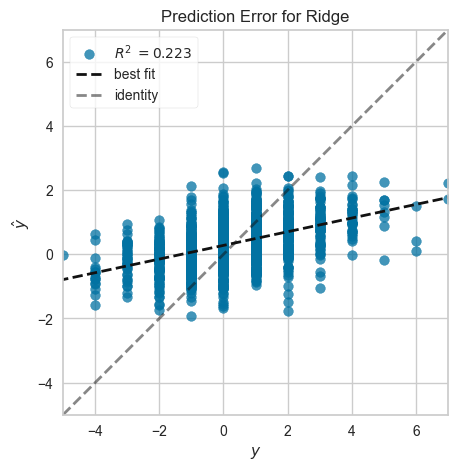
\includegraphics[width=\smallSize]{images/linearModelRidge.png}
    \caption{Ridge Regression: Prediccion del error}
    \label{Modelos-Lineales-Ridge-Prediccion-Error}
\end{figure}

De la misma forma que en el modelo de Regresión Lineal, en la Figura \ref{Modelos-Lineales-Ridge-Prediccion-Error} podemos ver como los resultados obtenidos no son demasiado satisfactorios. El valor de $R^2$, es el mismo que en la Regresión Lineal $0.223$, pero el valor de la validación cruzada ha mejorado levemente. En este caso, la media de las validaciónes cruzada es $0.218$. Y si queremos fijarnos en los valores individuales de cada validación, lo podemos encontrar en el Cuadro \ref{Modelos-Lineales-Ridge-Validacion-Cruzada}.

\begin{table}[h]
    \centering
    \begin{tabular}{lccccc}
        \textbf{Pliegue} & 1 & 2 & 3 & 4 & 5 \\
        \textbf{Resultado} & 0.25630708 & 0.12472019 & 0.25798172 & 0.17091906 & 0.28008048
    \end{tabular}
    \caption{Ridge Regression: Resultados Validación Cruzada}
    \label{Modelos-Lineales-Ridge-Validacion-Cruzada}
\end{table}

Para acabar, se ha visto que en este caso, el tiempo de entrenamiento es inferior al de la regression lineal, obteniendo un valor cercano a $0.002$ segundos de media. 